\usetikzlibrary{calc}
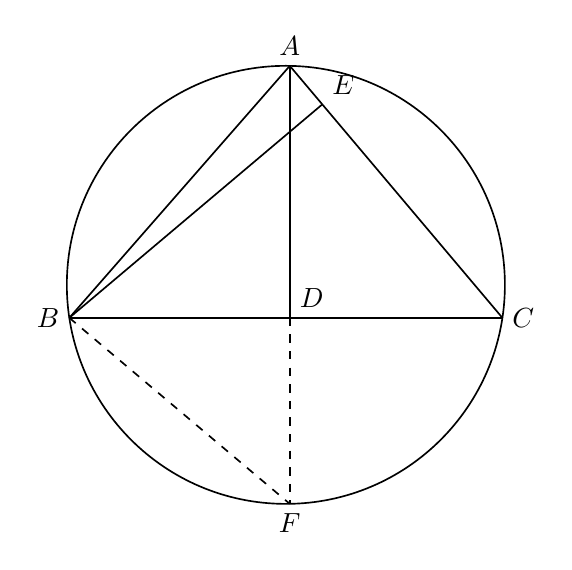
\begin{tikzpicture}[x=1cm,y=1cm,line width=.6pt,font=\normalsize]
\coordinate (O) at (0.25,0.4188);
\coordinate (A) at (0.3,3.2);
\coordinate (B) at (-2.5,0);
\coordinate (C) at (3,0);
\coordinate (D) at (0.3,0);
\coordinate (F) at (0.3,-2.3625);
\coordinate (E) at (0.7128,2.7108);
\draw[black] (O) circle[radius=2.7817cm];
\draw[black] (A)--(B);
\draw[black] (A)--(C);
\draw[black] (B)--(C);
\draw[black] (A)--(D);
\draw[black,dashed] (D)--(F);
\draw[black] (B)--(E);
\draw[black,dashed] (B)--(F);
\node[above] at (A) {$A$};
\node[left] at (B) {$B$};
\node[right] at (C) {$C$};
\node[above right] at (D) {$D$};
\node[above right] at (E) {$E$};
\node[below] at (F) {$F$};
\end{tikzpicture}
